% Licensed to the Apache Software Foundation (ASF) under one or more
% contributor license agreements. See the NOTICE file distributed with
% this work for additional information regarding copyright ownership.
% The ASF licenses this file to You under the Apache License, Version 2.0
% (the ``License''); you may not use this file except in compliance with
% the License. You may obtain a copy of the License at
%
% http://www.apache.org/licenses/LICENSE-2.0
%
% Unless required by applicable law or agreed to in writing, software
% distributed under the License is distributed on an ``AS IS'' BASIS,
% WITHOUT WARRANTIES OR CONDITIONS OF ANY KIND, either express or implied.
% See the License for the specific language governing permissions and
% limitations under the License.

\subsubsection{JDBC Job Options}

You must fill in the ``Scheduling,'' ``Queries,'' and ``Security''
tabs to configure a JDBC job.

\bigimage{JDBC-edit-job-tab3}

\ifJDBCGuide
% Licensed to the Apache Software Foundation (ASF) under one or more
% contributor license agreements. See the NOTICE file distributed with
% this work for additional information regarding copyright ownership.
% The ASF licenses this file to You under the Apache License, Version 2.0
% (the ``License''); you may not use this file except in compliance with
% the License. You may obtain a copy of the License at
%
% http://www.apache.org/licenses/LICENSE-2.0
%
% Unless required by applicable law or agreed to in writing, software
% distributed under the License is distributed on an ``AS IS'' BASIS,
% WITHOUT WARRANTIES OR CONDITIONS OF ANY KIND, either express or implied.
% See the License for the specific language governing permissions and
% limitations under the License.

\begin{itemize}
\label{scheduling}

\item \textbf{Schedule type:} Whether you want to scan every document
once or dynamically recrawl content in your repository. 

When scanning every document once, the crawler marks all documents that
have been previously crawled in this job as potentially to be deleted,
adds all seed documents to its queue and marks them as pending, processes
pending documents, marking them completed as they are ingested, and then
deleted all of the documents that were not recrawled. A document might
not be recrawled because it no longer exists, or the job specification
might have been changed to no longer include the document.

When dynamically recrawling documents, the crawler does not start by
marking all documents as potentially deletable; instead, it begins with
all of the seed documents, and continues adding to its list, periodically
re-adding the initial seed documents. If a document is removed from the
source, it will expire in the expiration interval (see below).

\item \textbf{Expiration Interval (if continuous):} The length of the
interval (in minutes) that the appliance will retain a document
crawled by this job after the document no longer appears in the
repository. After this interval, the missing document will be removed
from the appliance's index and archive. Leave the expiration interval
blank to keep missing documents indexed in GTS.

\item \textbf{Recrawl interval:} If you are dynamically recrawling
documents, how long, in minutes, the crawler should wait before
crawling documents a second time.

\item \textbf{Reseed interval:} If you are dynamically recrawling
documents, how long, in minutes, the crawler should wait before
looking for new documents to crawl. \ifMeridioGuide This connector
identifies all documents for ingestion through seeding; if the reseed
interval is infinite, the job will not ingest documents placed in the
repository during run time. (The job automatically reseeds whenever it
is started.) The default interval of 60 minutes is an appropriate
reseed rate. \fi \ifFilenetGuide This connector identifies documents
for ingestion during seeding. If you change the document inclusion
criteria, reseeding is required to identify new documents. Similarly,
documents placed in the repository while the job is running will not
be identified until the crawl is reseeded.  (The job automatically
reseeds whenever it is started.) The default interval of 60 minutes is
an appropriate reseed rate. \fi

\item \textbf{Scheduled time:} Allows you to define a time you wish
the job to run using a series of selection boxes. The first box refers
to the day of the week you wish the job to run, with an option to have
the job run any day of the week. The second box allows you to select
the start hour, with an option to start the job at any hour. The third
box allows you to specify which minute after the hour that you wish
the job to start. The fourth box allows you to specify what months of
the year you wish the job to run, with an option for the job to run
any month. The last box allows you to specify the day of the month you
wish the job to start, including any day of month.


You can scroll through each of the five boxes in this setting using
the arrow keys on your keyboard or by using the scroll bar on the
right side of the box.  If you want to select more than one value,
hold down control as you scroll and click the values that you want to
select. This allows you to define multiple windows with the same
length, for example by selecting Monday, Wednesday, and Friday at the
same time.

\item \textbf{Maximum run time:} The longest you will allow the job to
run, in minutes. For example, if you want to start a job at 2 AM but
force it to stop at 8 AM so that users have access to the repository,
you should set this value to 360 minutes. If the job is not complete by the
end time, documents that have already been found will be indexed, and
the rest of the crawl will continue at the beginning of the next
schedule interval. 

When you have defined the scheduled time and assigned a maximum run
time, click on the ``Add Scheduled Time'' button. A new schedule box
will appear below the scheduled time, allowing you to create
additional scheduled run times.

Here is a sample schedule for a job that will run every
Monday from 2 am to 6 am:

\begin{changemargin}{-.3in}{0in} 
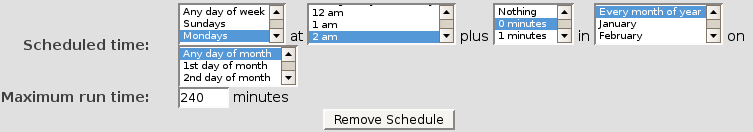
\includegraphics[width=300pt]{sample-schedule}
\end{changemargin}

If you do not have at least one scheduled time, the job will
only run when run manually (see page \pageref{ManageJobs}), and will
not automatically update the index on the appliance based on changes
to the repository.

You can remove a scheduled time by clicking the ``Remove Schedule''
button.

\end{itemize}

\fi

\ifCombinedConnectorGuide
This tab presents scheduling options. Here you can generate one or
more scheduled run times for the job. For a complete description of
the scheduling options, see the description starting on page
\pageref{scheduling}.
\fi

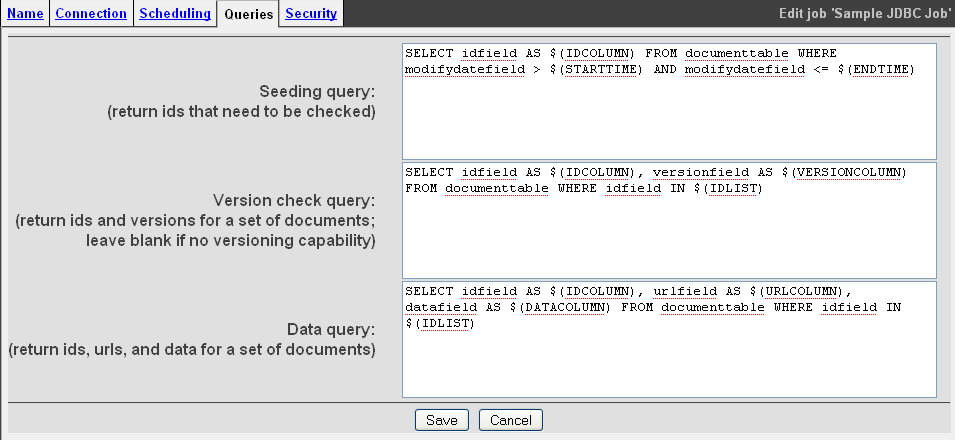
\includegraphics[width=300pt]{JDBC-edit-job-tab4}

In each of the three fields, you will need to construct an appropriate
SQL query. The sample queries shown include helper strings of the form
\command{\$(HELPER)} used by the connector, which are explained as they
appear.

\begin{itemize}

\item \textbf{Seeding Query:} The seeding query should return the
identifiers of documents in the repository that should be checked
against the files indexed in the GTS database. These identifiers
should be returned in a result-set as a column named
\command{\$(IDCOLUMN)}. The sample query shown above reads:

\begin{console}
SELECT idfield AS \$(IDCOLUMN) FROM documenttable WHERE modifydatefield
> \$(STARTTIME) AND modifydatefield <= \$(ENDTIME)

\end{console}

In this sample seeding query, identifiers from \command{idfield} for
entries from table \command{documenttable} are returned as a column
named \command{\$(IDCOLUMN)}. This example uses a \command{WHERE}
expression to limit the returned identifiers to entries with a
modified date, \command{modifydatefield}, in the range specified by
\command{\$(STARTTIME)} to \command{\$(ENDTIME)}. The time range spans
from the last time the job was run to the current start time, as
maintained by the GTS appliance. Time filtering is not a required part
of this query, but it helps reduce the number of documents being
passed to the ingestion interface by filtering out documents that have
not been modified since the last time the job was run.

A seeding query must be included. The seeding query must return a
column named \command{\$(IDCOLUMN)} as part of its result-set.

\note{Use caution when constructing queries that include time-based
components. \command{\$(STARTTIME)} and \command{\$(ENDTIME)} provide
times in milliseconds since epoch. If the modified date field is not
in this unit, the seeding query may not select the desired document
identifiers. You should convert \command{\$(STARTTIME)} and
\command{\$(ENDTIME)} to the appropriate timestamp unit for your system.

The following table gives several sample query fragments that can be
used to convert the helper strings \command{\$(STARTTIME)} and
\command{\$(ENDTIME)} into other date and time types. The first column names
the SQL database type that the following query phrase corresponds to,
the second column names the output data type for the query phrase, and
the third gives the query phrase itself using \command{\$(STARTTIME)}
as an example time in milliseconds since epoch. These query phrases
are intended as guidlines for creating an appropriate query phrase in
each language. Each query phrase is designed to work with the most
current version of the database software available at the time of
publishing for this document. If your modified date field is not of
the type given in the second column, the query phrase may not provide
an appropriate output for date comparisons.}

% Licensed to the Apache Software Foundation (ASF) under one or more
% contributor license agreements. See the NOTICE file distributed with
% this work for additional information regarding copyright ownership.
% The ASF licenses this file to You under the Apache License, Version 2.0
% (the ``License''); you may not use this file except in compliance with
% the License. You may obtain a copy of the License at
%
% http://www.apache.org/licenses/LICENSE-2.0
%
% Unless required by applicable law or agreed to in writing, software
% distributed under the License is distributed on an ``AS IS'' BASIS,
% WITHOUT WARRANTIES OR CONDITIONS OF ANY KIND, either express or implied.
% See the License for the specific language governing permissions and
% limitations under the License.

%BEGIN LATEX
\ifBigMargins\begin{changemargin}{-1.5in}{0in}\fi
\ifLittleMargins\begin{changemargin}{-.75in}{0in}\fi
%END LATEX

\begin{tabular}{|p{1in}|p{1in}|p{3.5in}|}

\hline

\textbf{Database Type}&\textbf{Date Type}&\textbf{Sample Query Phrase}\\

\hline

Oracle & \textit{date} & \command{ TO\_DATE ( '1970/01/01:00:00:00',
'yyyy/mm/dd:hh:mi:ss') + ROUND (\$(STARTTIME)/86400000)}\\

%Oracle & \textit{date} & \command{ TO_DATE ( '1970/01/01:00:00:00', 'yyyy/mm/dd:hh:mi:ss') + ROUND (\$(STARTTIME)/86400000)}\\

\hline

Oracle & \textit{timestamp} & \command{TO\_TIMESTAMP('1970-01-01 00:00:00')
+ interval '\$(STARTTIME)/1000' second}\\

\hline

Postgres SQL & \textit{timestamp} & \command{date '1970-01-01' + interval
'\$(STARTTIME) milliseconds'}\\

\hline

MS SQL Server ($>$6.5) & \textit{datetime} & \command{DATEADD(ms,
\$(STARTTIME), '19700101') }\\

\hline

Sybase (10+) &  \textit{datetime} &\command{DATEADD(ms,
\$(STARTTIME), '19700101') }\\

\hline

\end{tabular}
%BEGIN LATEX
\ifBigMargins\end{changemargin}\fi
\ifLittleMargins\end{changemargin}\fi
%END LATEX


\item \textbf{Version Check Query:} If your document system has
versioning capabilities, a version check query should be used to
filter documents based on version. The sample version query shown
above reads:

\begin{console}
SELECT idfield AS \$(IDCOLUMN), versionfield AS \$(VERSIONCOLUMN) FROM
documenttable WHERE idfield IN \$(IDLIST)
\end{console}

The sample query returns a column
named \command{\$(IDCOLUMN)} of identifiers from \command{idfield} and a
column named \command{\$(VERSIONCOLUMN)} of version numbers from
\command{versionfield} from entries in the table \command{documenttable}
whose identifiers were passed to this query by the job process using
the input \command{\$(IDLIST)}.

A version check query is not required. If your document system does
not have versioning capability, leave this query blank.

\item \textbf{Data Query:} A data query returns the identifiers, URLs,
and data for a document. The sample data query shown above reads:

\begin{console}
SELECT idfield AS \$(IDCOLUMN), urlfield AS \$(URLCOLUMN), datafield AS
\$(DATACOLUMN) FROM documenttable WHERE idfield IN \$(IDLIST)
\end{console}

This sample data query returns three columns, a column named\linebreak
\command{\$(IDCOLUMN)} of identifiers from \command{idfield}, a column
named \command{\$(URLCOLUMN)} of document URLs from \command{urlfield},
and a column named \command{\$(DATACOLUMN)} of document contents from
\command{datafield}. These outputs are generated from entries in the table
\command{documenttable} whose identifiers were passed to this query by
the job process using the input \command{\$(IDLIST)}.

The data query is required. This query passes the documents and
associated information to the ingestion interface for either initial
ingestion or re-ingestion.

\end{itemize}

When possible, filter the files passed to the ingestion interface by
way of version, modification time, or other methods to reduce the
number of files that are re-ingested unnecessarily. This can
significantly improve the performance of the ingestion.

The exact entry form of helper strings varies depending on the type of
database being used. In the case of Postgres SQL, MS SQL Server, and
Sybase, the helper strings should just be entered as shown in the
sample queries, as \command{\$(HELPER)}. In the case of Oracle, the
helper strings naming columns should be enclosed in double
quotation marks, as \command{\char34\$(IDCOLUMN)\char34},
\command{\char34\$(VERSIONCOLUMN)\char34},\linebreak
\command{\char34\$(URLCOLUMN)\char34}, and
\command{\char34\$(DATACOLUMN)\char34}, while the helper strings
\command{\$(IDLIST)}, \command{\$(STARTTIME)}, and
\command{\$(ENDTIME)} should be left as shown.

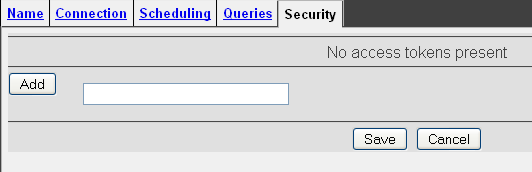
\includegraphics[width=300pt]{JDBC-edit-job-tab5}

If you wish to enable security, the user permissions you enter here will
be ingested with each document in this job. Otherwise, all documents in
this job will be ingested without permissions.

\item \textbf{Access Tokens:} To specify your own ACLs for files ingested
through this job, you can specify enter one or more ACL identifiers into
this field and click the ``Add'' button. The ACL identifiers will appear
in a list. You can continue to add more ACL identifiers using the ``Add''
button, or remove them using the ``Delete'' button that appears next to
each ACL identifier.

After entering this information, you will be taken to the status page
for this job:

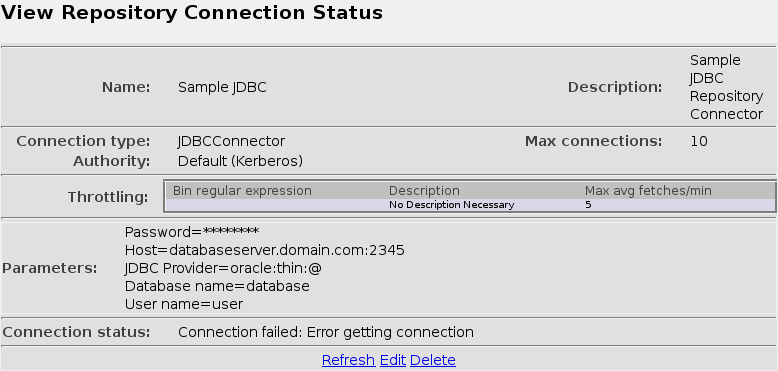
\includegraphics[width=300pt]{JDBC-view-job-status}
